\documentclass[
    11pt,
    spanish,
    a4paper
]{article}
\usepackage[utf8]{inputenc}
\usepackage[spanish]{babel}
\usepackage{authoraftertitle}
\usepackage{booktabs}
\usepackage{caption}
\usepackage{float}
\usepackage{graphicx}
\usepackage{listings}
\usepackage{verbatim}
\usepackage{amsmath}

\def\doctype{Trabajo práctico}
\title{Markov y PFD}
\author{Gonzalo Nahuel Vaca}

\begin{document}

\makeatletter
\begin{titlepage}
	\begin{center}
		\vspace*{1cm}

		\Huge
		\textbf{\doctype}
		\vspace{0.5cm}

		\LARGE
		\@title
		\vspace{0.5cm}

		\textbf{Introducción a los sistemas críticos}

		\vspace{1.5cm}

		\textbf{\@author}

		\vspace{1.5cm}

		
\includegraphics[width=0.8\textwidth]{img/logoFIUBA.pdf}

		\vfill
		Maestría en Sistemas Embebidos\\
		Universidad de Buenos Aires\\
		Argentina\\
		\today
	\end{center}
\end{titlepage}
\makeatother
\newpage

\section{Diagrama de transición de estados}

\begin{figure}[htbp]
	\centering
	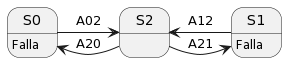
\includegraphics[width=0.5\textwidth]{img/diagrama_estados.png}
	\caption{Diagrama de estados.}
	\label{fig:diagrama_estados}
\end{figure}

Donde:

$ A_{21} = \lambda_1 $; Tasa de falla del componente 1

$ A_{12} = \mu_1 $; Tasa de reparación del componente 1

$ A_{20} = \lambda_2$; Tasa de falla del componente 1

$ A_{02} = \mu_2$; Tasa de reparación del componente 1

Cuando un componente no presta servicio se supone que no se expone a desgastes ni esfuerzos.
Esto significa que las transiciones de estados 1 a 0 o 0 a 1 es 0.
Finalmente $ A_{01} = A_{10} = 0 $.

\section{Ecuación matricial del proceso de Markov}

$$ \dot{P(t)} = P(t) . A $$

Donde:
\begin{itemize}
	\item $ P(t) $: matriz de estados cuyas entrada es la probabilidad de transición del proceso Markov.
	\item $ A $: matriz de tasas de transición.
\end{itemize}

Alternativamente se puede expresar de la siguiente manera:

\begin{equation}
	[\dot{P_0(t)},\dot{P_1(t)},\dot{P_2(t)}] =
	\begin{pmatrix}
		P_{00}(t) & P_{01}(t) & P_{02}(t) \\
		P_{10}(t) & P_{11}(t) & P_{12}(t) \\
		P_{20}(t) & P_{21}(t) & P_{22}(t)
	\end{pmatrix} *
	\begin{pmatrix}
		a_{00} & a_{01} & a_{02} \\
		a_{10} & a_{11} & a_{12} \\
		a_{20} & a_{21} & a_{22}
	\end{pmatrix}
\end{equation}

En sistemas estacionarios se debe satisfacer:

\begin{equation}
	[0,0,0] = [\dot{P_0(t)},\dot{P_1(t)},\dot{P_2(t)}] *
	\begin{pmatrix}
		-\mu_2    & 0         & \mu_2                   \\
		0         & -\mu_1    & \mu_1                   \\
		\lambda_2 & \lambda_1 & (\lambda_1 + \lambda_2)
	\end{pmatrix}
\end{equation}

\section{Calcular:}

\subsection{Probabilidad de que el sistema esté en cada uno de los estados, $P_j$.}

$$ P_0 + P_1 + P_2 = 1 $$

$$ -\mu_2 * P_0 + \lambda_2 * P_2 = 0 $$
$$ P_0 = \frac{\lambda_2}{\mu_2} * P_2 $$

$$ -\mu_1 * P_1 + \lambda_1 * P_2 = 0 $$
$$ P_1 = \frac{\lambda_1}{\mu_1} * P_2 $$

$$ P_1 = P_2 = 0,069 $$

\subsection{Indisponibilidad del sistema}

$$ A_s = P_2 = \frac{\mu_1*\mu_2}{\lambda_1*\mu_2+\lambda_2*\mu_1+\mu_1*\mu_2} = 0,862 $$

$$ \bar{A_s} = 1 - A_s = 0,138 $$

\subsection{Duración media de que el sistema permanezca en cada uno de los estados}

La frecuencia de fallas es igual a la frecuencia de visitas.

$$ W_f = V_2 = P_2 * (\lambda_1 + \lambda_2) = 0,01724 $$

\subsection{Tiempo medio entre fallas del sistema}

$$ MTBF_s = \frac{1}{W_f} = 58 $$

\subsection{Tiempo medio de falla del sistema}

$$ \theta_F = \frac{1 - A_s}{W_f} $$
$$ \theta_F = \frac{1 - 0.862}{0.01724} $$
$$ \theta_F = 8 $$

\section{Analice otro diagrama de transición de estados si los dos componentes estuvieran en paralelo}

\begin{figure}[htbp]
	\centering
	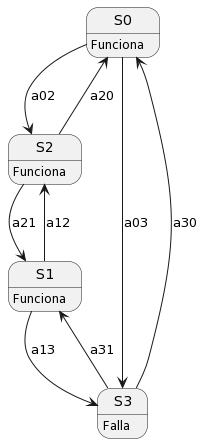
\includegraphics[width=0.3\textwidth]{img/diagrama_estados_2.png}
	\caption{Diagrama ejercicio 4.}
	\label{fig:diagrama_estados_2}
\end{figure}

$ a_{21} = \lambda_1 $, Tasa de falla del componente 1

$ a_{12} = \mu_1 $, Tasa de reparación del componente 1

$ a_{20} = \lambda_2 $, Tasa de falla del componente 2

$ a_{02} = \mu_2 $, Tasa de reparación del componente 2

$ a_{13} = \lambda_2 $, Tasa de falla del componente 2

$ a_{31} = \mu_2 $, Tasa de reparación del componente 2

$ a_{03} = \lambda_1 $, Tasa de falla del componente 1

$ a_{30} = \mu_1 $, Tasa de reparación del componente 1

\end{document}